\documentclass[a4paper,10pt]{article}

\usepackage{xunicode,xltxtra,url,parskip}
\RequirePackage{color,graphicx}
\usepackage[usenames,dvipsnames]{xcolor}
\usepackage{framed}

% Custom section.
\usepackage{titlesec}

% Document margins.
\usepackage{geometry}
\geometry{left = 1.0in,right = 1.0in,top = 1.0in,bottom = 1.0in}

% Setup hyperref package, and colours for links
\usepackage{hyperref}
\definecolor{linkcolour}{rgb}{0,0.0,0.0}
\hypersetup{colorlinks,breaklinks,urlcolor=linkcolour,linkcolor=linkcolour}

\titleformat{\section}{\Large\scshape\raggedright}{}{0em}{}[\titlerule]
\titlespacing{\section}{0pt}{3pt}{3pt}

% Figures directory.
\graphicspath{{figures/}}

% Footer
\usepackage{fancyhdr}
\pagestyle{fancy}
\fancyhf{}
% Remove line for header.
\renewcommand{\headrulewidth}{0pt}
\fancyfoot[C]{
    \raisebox{-2pt}{
\includegraphics[height=12pt]{github.png}}
    \href{https://github.com/faku99}{faku99}
    %\hspace*{12pt}
    %\raisebox{-2pt}{
\includegraphics[height=12pt]{www.png}}
    %\href{https://elisei.ch}{elisei.ch}
    \hspace*{12pt}
    \raisebox{-2pt}{
\includegraphics[height=12pt]{linkedin.png}}
    \href{https://www.linkedin.com/in/lucas-elisei-83667ab5}{Lucas Elisei}
}


\begin{document}

\begin{minipage}{0.6\textwidth}
    {\huge \textsc{Lucas Elisei}} \\
    \\
    11\textsuperscript{th} March 1995 \\
    \\
    Chemin Près-les-Bois 1F \\
    1066 Epalinges, Switzerland \\
    \\
    +41 79 137 66 92 (Swizerland) \\
    +33 6 42 40 31 25 (France) \\
    \href{mailto:elisei.lucas@gmail.com}{elisei.lucas@gmail.com}
\end{minipage} %
\begin{minipage}{0.4\textwidth}
    \begin{flushright}
        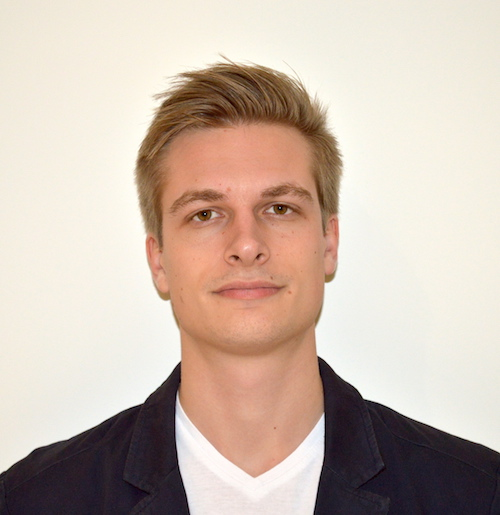
\includegraphics[width=0.6\textwidth]{photo.jpg}
    \end{flushright}
\end{minipage}

\vspace*{0.5cm}

\iffalse
\begin{framed}
    \centering
    \large{\textsc{
        Master student looking for a summer internship
    }}
\end{framed}
\else
\vspace*{1.2cm}
\fi

\section{Education}

\begin{tabular}{lp{12cm}}
    \textsc{Sept 2018} & Master of Science in Engineering, Embedded Systems, \textbf{HES-SO}, Lausanne \\
    to \textsc{June 2020} \\
    \\
    \textsc{Sept 2019} & Master thesis: ``High Performance Overlays for FPGA'' \\
    to \textsc{Feb 2020} \\
    \\
    \textsc{Feb 2019} & Semester project: ``FPGA-based Accelerator for Machine Learning Inference'' \\
    to \textsc{June 2019} \\
    \\
    \textsc{Sept 2015} & Bachelor of Engineering in Embedded Systems, \textbf{HEIG-VD}, Yverdon \\
    to \textsc{July 2018} & Thesis: ``Just-in-Time Recompilation and Optimization of Compiled Binaries'' \\
    \\
    \textsc{Sept 2013} & Propedeutics, \textbf{Swiss Federal Institute of Technology (EPFL)}, Lausanne \\
    to \textsc{July 2015} \\
    \\
    \textsc{June 2013} & Scientifical \textit{Baccalauréat} (mathematics speciality), mention ``Bien'' with physics \\
    \hspace*{2.3cm} & taught in English.
\end{tabular}

\section{Projects}

\begin{tabular}{p{2.3cm}p{12cm}}
    \textsc{Stereo}
    & Flutter library for playing music from a file. \\
    \\

    \textsc{Commusica}
    & Java application for sharing music during an event. \\
    \\

    \textsc{Goodges}
    & iOS extension for jailbroken devices. Radically changes the way notification badges are displayed on the homescreen. \\
    \\

    \textsc{Imhof}
    & Draw topographic map of cities from OpenStreetMap data. \\
    \\

    \textsc{PageRank}
    & Recommendation algorithm.
\end{tabular}

\section{Work Experience}

\begin{tabular}{lp{12cm}}
    \textsc{Summer 2019}
    & Summer Internship at \textsc{REDS Institute}, Yverdon \\
    & \footnotesize{Deployment of a Deep Neural Network model on FPGA in a Software-Defined Radio system.} \\
    \\

    \textsc{Summer 2017}
    & Interim at \textsc{Nestlé}, Orbe \\
    & \footnotesize{Quality controls on Dolce Gusto products.} \\
    \\

    \textsc{Summer 2016}
    & Summer Internship at \textsc{Itecor}, Vevey \\
    \hspace*{2.3cm} & \footnotesize{Development of a mobile application for iOS, Android and Windows platforms. Acknowledged for my professionalism, my integration in a international environment and my English communication skills.} \\
    \\

    \textsc{Summer 2015}
    & Summer Internship at \textsc{Y-Parc}, Yverdon \\
    & \footnotesize{Development of a web application whose aim is to create and manage multiple-choice tests. Acknowledged for my positive attitude, my engagement and my organization.} \\
    \\

    \textsc{Feb 2015} & Interim at \textsc{Nestlé}, Orbe \\
    & \footnotesize{Life-cycle tests on Nescafé \textit{Dolce Gusto} machines for sale.} \\
    \\

    \textsc{Summer 2013} & Interim at \textsc{Nestlé}, Orbe \\
    & \footnotesize{Quality controls on Nescafé and Nespresso products.}
\end{tabular}

\section{Languages}

\begin{tabular}{p{2.3cm}l}
    \textsc{French}  & Mothertongue \\
    \textsc{Italian} & Mothertongue \\
    \textsc{English} & Fluent (C1 Level)\\
\end{tabular}

\section{Skills}

\textbf{Computer skills} \\
\begin{tabular}{p{2.3cm}l}
    Basic & \textsc{Excel}, \textsc{PowerPoint}, \textsc{JavaScript} \\
    Intermediate & \textsc{Assembly}, \textsc{C++}, \textsc{Java}, \LaTeX, \textsc{SystemVerilog}, \textsc{Quartus}, \textsc{Vivado}, \textsc{Python}  \\
    Advanced & \textsc{C}, \textsc{Dart}, \textsc{Git}, \textsc{SoC/FPGA}, \textsc{VHDL} \\
    \\
\end{tabular}

\parbox{2.8cm}{\textbf{Soft skills}} Autonomous, ability to adapt, organized and quick learner.


\section{Interests and Activities}

Technology, Open-Source, Programming \\
Music, Travelling

\end{document}
